\subsection{Exploratory checks of ranking, target entropy and temporal aggregation}
\label{sec:final-diagnostics}

These analyses use retained predictions after earlier outcomes were known. We applied the centered logit normalization studied by Xia et al.~\cite{xia2025smoothing}. For saved positive probabilities, let $z_c=\log p_c-K^{-1}\sum_j\log p_j$ and rank by $s_a=\max_c z_c/\lVert z\rVert_a$. The unknown softmax offset cancels, recovering centered logits algebraically; rounded float32 probabilities only approximate the original values. No saved probability required zero clipping. The exponent $a\in\{1,1.5,2,3,4,6,8,16\}$ minimizes mean all-prefix calibration risk (AURC) for complete-vote disagreement, with the first candidate resolving ties. Calibration selects parameters; test results remain exploratory. This adapts the published score to our endpoint rather than reproducing its original experiments.

Across all 48 original retained states, the best normalized score had worse calibration AURC than MSP. A calibration-only choice between MSP and normalization therefore retained MSP in every case. Normalization alone reduced the selected Swin-T Soft--Uniform advantage from $-0.378$ to $-0.223$ pp; ResNet-18 remained in the opposite direction (Table~\ref{tab:ranking-followup}). The small Swin-T contrast persists under this examined correction, although the calibration procedure selects MSP throughout. Class predictions remain unchanged, and full-coverage risk is score-invariant. These results concern crowd disagreement rather than the ordinary classification-error endpoint studied by Xia et al.

\begin{table}[!htbp]
\centering
\caption{Soft-minus-Uniform disagreement at 80\% coverage, in percentage points. Each score selects its own images. Centered normalization uses calibration-selected exponents; the calibration choice between scores equals MSP for all 48 original states. These are exploratory means over three fitted seed pairs.}
\label{tab:ranking-followup}
\begin{tabular}{llrr}
\toprule
Backbone & State & MSP & Centered norm \\
\midrule
Swin-T & selected & -0.378 & -0.223 \\
Swin-T & epoch12 & -0.317 & -0.122 \\
ResNet-18 & selected & +0.173 & +0.355 \\
ResNet-18 & epoch12 & +0.170 & +0.459 \\
\bottomrule
\end{tabular}

\end{table}

The controls also differ in measurable training-target properties. On the 28,557 positive-mass training images, mean entropy is 0.5067 nats for Soft, 0.8002 for Uniform and 0.7727 for Tie-Uniform. After weighting by supported vote mass, the corresponding values are 0.4949, 0.7812 and 0.7553. Their weighted class-marginal L1 differences from Soft are 0.1197 and 0.1032. These quantities substantiate the remaining entropy and class-proportion differences; they do not identify a causal minority-category mechanism. The 152 zero-mass images contribute no supervised target loss.

For all 36 external states, we compared the original eight-frame mean with the fixed middle four sampled positions (2--5, zero-based). Positions were determined chronologically within each clip before averaging; the window was not tuned against outcomes. We reranked all 1,440 clips separately under each aggregation and retained 1,152 at 80\% coverage. Reconstructing the original eight-frame means exactly matched every stored clip probability vector. For selected Swin-T Soft, the middle window reduced mean raw-reference disagreement from 68.37\% to 63.84\%, and calm-merged disagreement from 60.72\% to 56.71\% (Fig.~\ref{fig:aggregation-followup}). Its neutral prediction fraction decreased from 68.37\% to 55.09\%. The raw Soft--Uniform contrast remained positive ($+0.61$ versus $+0.59$ pp); the calm-merged contrast changed from $+0.10$ to $-0.21$ pp with mixed seed directions. Temporal aggregation affects absolute transfer performance substantially without establishing a stable supervision advantage.

\begin{figure}[!htbp]
\centering
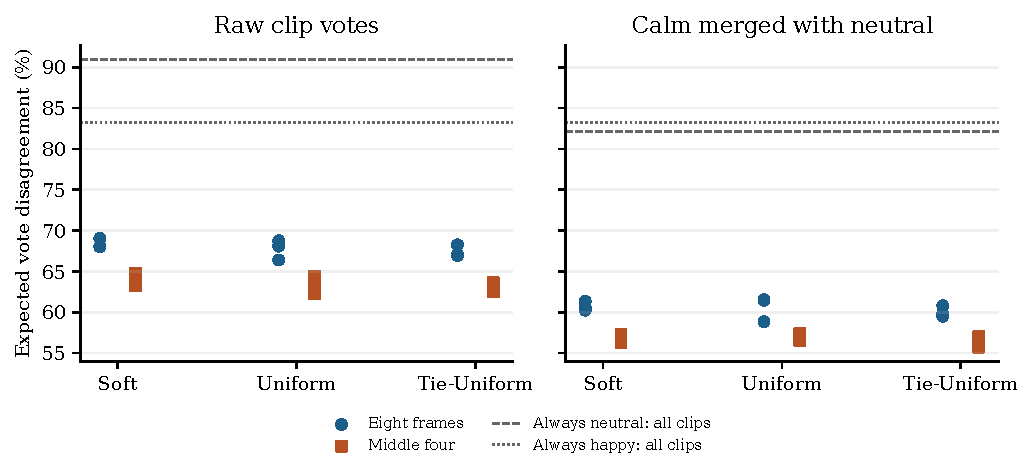
\includegraphics[width=\linewidth]{final_revision_2026_10_20/source/figures/ExternalAggregation.pdf}
\caption{Exploratory temporal aggregation for validation-selected Swin-T. Points show three seeds at 80\% coverage under each model's own MSP ranking. Reference lines show constant-category predictions on all 1,440 clips, a different population from the selected points. Exact accepted-set references are reported separately. The middle window is fixed, and clip-level human votes provide no frame-level ground truth.}
\label{fig:aggregation-followup}
\end{figure}

Always predicting neutral gives 90.94\% disagreement on all clips under raw scoring and 82.18\% after merging calm; always predicting happy gives 83.23\% under either reference. On the exact accepted sets of the original selected Swin-T Soft models, always-neutral risks average 88.80\% raw and 78.12\% merged; always-happy risk is 79.45\% under both references. The models outperform these simple references but still transfer poorly. Constants have no confidence ranking. Per-seed values, both backbones and states, exact-set references and calculation audits accompany the release. The checks narrow possible explanations without identifying a unique cause or establishing communication benefit.
